%-------------------------------------------------------------------------------
% Document & Package declarations
%-------------------------------------------------------------------------------

\documentclass[a4paper, 10pt, conference]{ieeeconf}
\usepackage{graphicx}
\usepackage[colorlinks=true, allcolors=black]{hyperref}
\usepackage{tabularx}

%% Language and font encodings
\usepackage[english]{babel}
\usepackage[utf8x]{inputenc}
\usepackage[T1]{fontenc}

%% Useful packages
\usepackage{amsmath}
\usepackage{graphicx}
\usepackage[colorinlistoftodos]{todonotes}
\usepackage[font=footnotesize,labelfont=bf]{caption}
\usepackage[font=footnotesize,labelfont=bf]{subcaption}

%% Packages for displaying source code
\usepackage{listings}
\usepackage{matlab-prettifier}
% \usepackage[framed,numbered,autolinebreaks,useliterate]{mcode}

\usepackage{float}


%%*************************************************************************
%% Legal Notice:
%% This code is offered as-is without any warranty either expressed or
%% implied; without even the implied warranty of MERCHANTABILITY or
%% FITNESS FOR A PARTICULAR PURPOSE!
%% User assumes all risk.
%% In no event shall IEEE or any contributor to this code be liable for
%% any damages or losses, including, but not limited to, incidental,
%% consequential, or any other damages, resulting from the use or misuse
%% of any information contained here.
%%
%% All comments are the opinions of their respective authors and are not
%% necessarily endorsed by the IEEE.
%%
%% This work is distributed under the LaTeX Project Public License (LPPL)
%% ( http://www.latex-project.org/ ) version 1.3, and may be freely used,
%% distributed and modified. A copy of the LPPL, version 1.3, is included
%% in the base LaTeX documentation of all distributions of LaTeX released
%% 2003/12/01 or later.
%% Retain all contribution notices and credits.
%% ** Modified files should be clearly indicated as such, including  **
%% ** renaming them and changing author support contact information. **
%%
%% File list of work: IEEEtran.cls, IEEEtran_HOWTO.pdf, bare_adv.tex,
%%                    bare_conf.tex, bare_jrnl.tex, bare_jrnl_compsoc.tex,
%%                    bare_jrnl_transmag.tex
%%*************************************************************************

%-------------------------------------------------------------------------------
% Document Configuration
%-------------------------------------------------------------------------------

\begin{document}
\title{Pattern Recognition - PCA and SVM for Facial Recognition}
\author{Michael~Hart and
        Meng~Kiang~Seah
\\
        Department of Electrical and Electronic Engineering,
        Imperial College London,
        SW7 2AZ
 \\
        E-mail: \{mh1613, mks211\}@imperial.ac.uk}
\date{\today}

%-------------------------------------------------------------------------------
% Plan on what to write
%-------------------------------------------------------------------------------

% See coursework instructions at:
% https://bb.imperial.ac.uk/bbcswebdav/pid-1001497-dt-content-rid-3367484_1/courses/DSS-EE4_68-16_17/PRCoursework1.pdf

%-------------------------------------------------------------------------------
% Information Banner
%-------------------------------------------------------------------------------

\maketitle

%-------------------------------------------------------------------------------
% Abstract
%-------------------------------------------------------------------------------

\begin{abstract}
\todo{Write abstract.} Lorem ipsum dolor sit amet, consectetur adipiscing elit. Vivamus feugiat metus id dictum venenatis. Etiam id luctus elit, quis tristique lacus. Ut tincidunt purus nec lacinia condimentum. Phasellus at est lacinia, porttitor massa at, vulputate nisl. Nullam turpis dolor, egestas nec enim ac, euismod congue nibh. Curabitur aliquet lacus vitae sem facilisis, quis luctus nisi tristique. Fusce odio risus, sagittis eu semper sit amet, pretium sit amet felis. Nunc a nunc ornare, tincidunt libero in, condimentum turpis.Lorem ipsum dolor sit amet, consectetur adipiscing elit. Vivamus feugiat metus id dictum venenatis. Etiam id luctus elit, quis tristique lacus. Ut tincidunt purus nec lacinia condimentum. Phasellus at est lacinia, porttitor massa at, vulputate nisl. Nullam turpis dolor, egestas nec enim ac, euismod congue nibh.
\end{abstract}

%-------------------------------------------------------------------------------
% Introduction
%-------------------------------------------------------------------------------
\section{Introduction}
Throughout this course, there are two methods of classifying data using pre-trained models that have explored. Principal Component Analysis (PCA) and Support Vector Machines (SVMs). These two methods are applied to the face data that is given. Each face is given as a 2561-by-1 column vector. These are the raw intensity vectors obtained by taking the pixel values of each image row by row and concatenating them. Each image given is a greyscale picture 42 pixels wide and 52 pixels high.

While regurgitating the theory presented in lectures in not the aim, it is necessary to establish some context for the work done.

\subsection{Principal Component Analysis}\label{sec:pcatheory}
Each image exists as a point in the $D$-dimensional space. The goal is to project these points onto a $M$-dimensional space (where $ M < D$), where this subspace contains the largest variance of the points. This is done by finding the eigenvalues and eigenvectors of the data's covariance matrix, $S$. The data is projected onto the largest $M$ eigenvectors chosen.

For classification, the Nearest Neighbour (NN) method is used. Each testing picture is also projected onto the subspace. This point is compared with the closest training point to it, and the testing picture is assigned the same class

\subsection{Support Vector Machines}\label{sec:svmtheory}
This is method involves creating a hyperplane in the $D$-dimensional space of the data, which separates the data into two classes. This is done by finding the plane in the space separates the data with the maximum distance from the training points closest to the boundary.

However, SVMs work for two classes only. To extend this to multiple classes, there are two ways. The first, one-versus-all, involves training each class's points against every other classes'. Thus, for $M$ classes, there are $M$ classes, there are $M$ SVMs, each tailored to each class. A test point is assigned the class of the SVM that determines it as a positive result.

The second is one-versus-one, which trains each class against every other class. This creates $\frac{M \times (M-1)}{2}$ SVMs. Each SVM votes on the class of a point, and the class with the most votes is assigned to the point.

% Plan for intro
% Probably going to be written at the end
% Introduce the concepts of PCA, SVMs, and classifiers in general
%
\section{Data Partitioning}
\todo{Too casual?}
A number of literature sources discuss the size and ratios of partitioning data for training and testing. They propose a range that extends from a 60\% training to 40\% testing ratio to one of 80\% to 20\%. Closer inspection of the data given to us in \texttt{face.math} shows that there are 520 pictures and 52 different classes. For each class, or each person, there are 10 images.

Weighing the need for enough training instances with enough testing instances, it was decided that a 70\% to 30\% training to testing ratio would be used. This would be across each class, with 7 training faces versus 3 testing faces for each class. The 3 testing instances were the 8th, 9th and 10th instances. As there is no ordering to the pictures in each class, there is no chance of an accidental bias.

This gives us 364 training instances with 156 testing ones. This partitioning is used for the remainder of this assignment.

\section{Principal Component Analysis}

% Training length is 364; test length is 156.
% Rank of AAT is 363
% Number of nonzero elements in AAT is 363
% Rank of ATA is 363
% Number of nonzero elements in ATA is 363

\subsection{PCA with $S = \frac{1}{N}AA^{T}$}
As mentioned in Section \ref{sec:pcatheory}, the first step in PCA is obtaining the data covariance matrix $S$. This can be done with the equation in the title. The $A$ matrix has 364 columns of training pictures of 2576 rows pixels each. It is obtained by subtracting the average training face (shown in Figure \ref{fig:meanface}) from each face.

Thus, $S$ has 2576 rows and columns. At first, using MATLAB to obtain the eigenvalues gives us 2756 values. However, closer inspection shows that the rank of $S$ is 363, meaning that they cannot be more than 363 non-zero eigenvalues. Indeed, rounding off the eigenvalues to 10 decimal places gives 363 non-zero values. This is most likely a floating precision issue.

\begin{figure}[h]
    \centering
    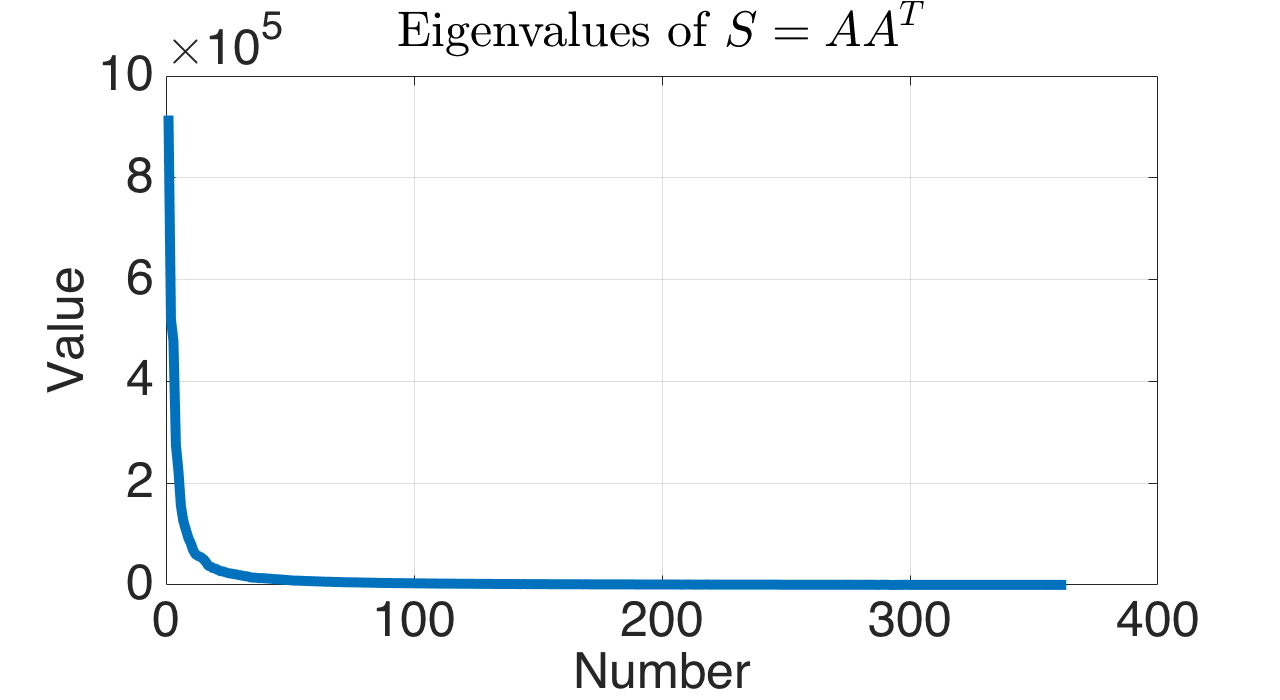
\includegraphics[width=0.5\textwidth]{src/S_eig_val_rounded.png}
    \caption{Eigenvalues from $S = AA^T$.}
    \label{fig:S_eig_val}
\end{figure}

The values of these eigenvalues are plotted in Figure \ref{fig:S_eig_val}. As can be seen, the values drop in an exponential manner. This is as was seen in the lecture slides. The largest eigenvalues have corresponding eigenvectors, or eigenfaces, and are the most common parts of the faces in the training set. Indeed, this method extracts the most important parts of the faces to use for recognition. The three main eigenfaces are shown in Figures \ref{fig:eigface1}, \ref{fig:eigface2}, and \ref{fig:eigface2}.

\begin{figure}[ht]
	\captionsetup[subfigure]{position=b}
        \centering
        \begin{subfigure}{0.2\textwidth}
                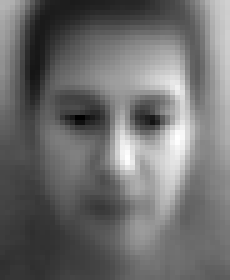
\includegraphics[width=\textwidth]{src/mean_face.png}
                \caption{The average testing face.}
                \label{fig:meanface}
        \end{subfigure}
        ~
        \begin{subfigure}{0.2\textwidth}
          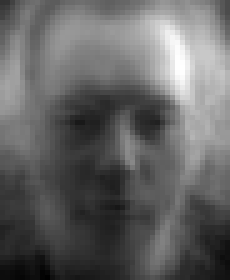
\includegraphics[width=\textwidth]{src/eigface1.png}
                \caption{The first eigenface.}
                \label{fig:eigface1}
        \end{subfigure}
        \\
        \begin{subfigure}{0.2\textwidth}
          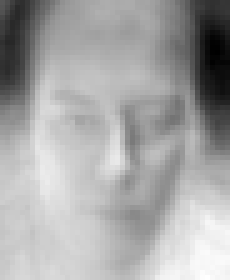
\includegraphics[width=\textwidth]{src/eigface2.png}
                \caption{The second eigenface.}
                \label{fig:eigface2}
        \end{subfigure}
        ~
        \begin{subfigure}{0.2\textwidth}
          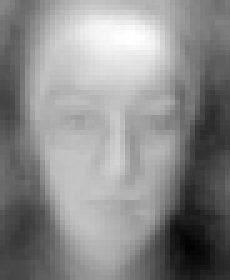
\includegraphics[width=\textwidth]{src/eigface3.png}
                \caption{The third eigenface.}
                \label{fig:eigface3}
        \end{subfigure}
	\caption{Mean face and some eigenfaces of $S = AA^T$ (visualisations of the eigenvectors).}
\end{figure}

\subsection{PCA with $S = \frac{1}{N}A^{T}A$}

\begin{figure}[h]
    \centering
    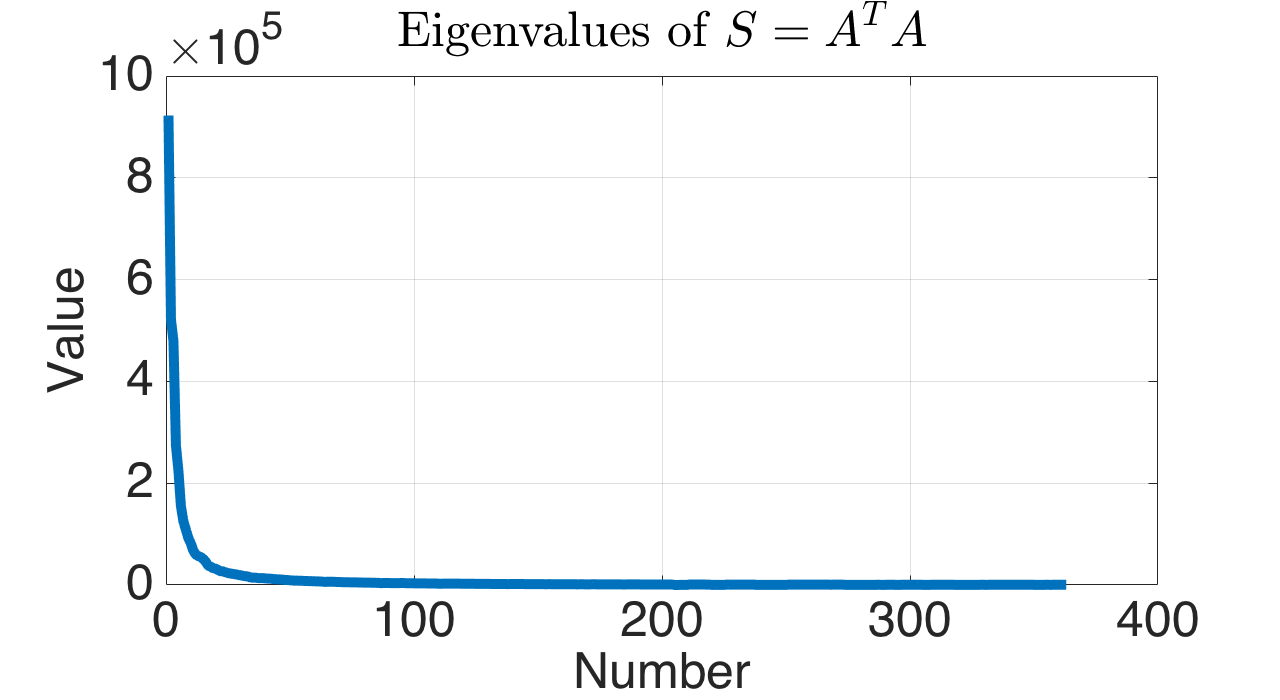
\includegraphics[width=0.5\textwidth]{src/S2_eig_val_rounded.png}
    \caption{Eigenvalues from $S = A^T A$.}
    \label{fig:S2_eig_val}
\end{figure}

$S = \frac{1}{N}A^{T}A$ is the alternative calculation method. From the lecture slides, the relationship between the eigenvalues and eigenvectors is known. The eigenvalues of $A^T A$ and $AA^T$ are actually identical. The eigenvectors of $AA^T$ ($u_i$) and $AA^T$ ($v_i$) are related by the equation $u_i = A v_i$. Figure \ref{fig:S2_eig_val} shows the eigenvalues and graphed in the same way as in Figure \ref{fig:S_eig_val}, and the trend is similar. Closer inspection in MATLAB showed that both contained the exact same values. For some context, the first 4 eigenfaces obtained through this method are shown. It is important to note that the eigenvectors have already been normalised.

\begin{figure}[ht]
	\captionsetup[subfigure]{position=b}
        \centering
        \begin{subfigure}{0.2\textwidth}
                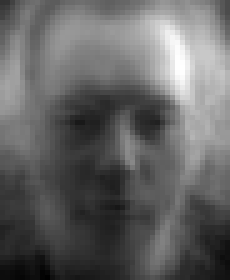
\includegraphics[width=\textwidth]{src/eigface4.png}
                \caption{The first eigenface.}
                \label{fig:eigface4}
        \end{subfigure}
        ~
        \begin{subfigure}{0.2\textwidth}
          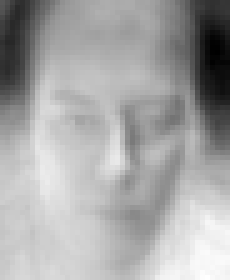
\includegraphics[width=\textwidth]{src/eigface5.png}
          \caption{The second eigenface.}
                \label{fig:eigface5}
        \end{subfigure}
        \\
        \begin{subfigure}{0.2\textwidth}
          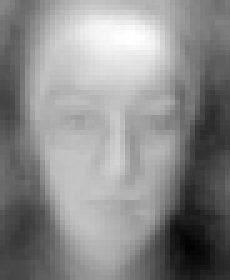
\includegraphics[width=\textwidth]{src/eigface6.png}
          \caption{The third eigenface.}
                \label{fig:eigface6}
        \end{subfigure}
        ~
        \begin{subfigure}{0.2\textwidth}
          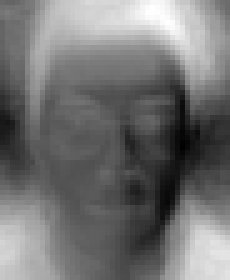
\includegraphics[width=\textwidth]{src/eigface7.png}
                \caption{The fourth eigenface.}
                \label{fig:eigface7}
        \end{subfigure}
	\caption{Some eigenfaces from $S = A^T A$.}
\end{figure}

Supplementing visual confirmation to the confirmation in MATLAB, it can be seen that most of the eigenvectors are the same. However, there are number of unusual cases where the sign of the eigenvector is reversed. This is peculiar, as there is no mention of such an occurrence in the notes. In fact, the mathematics presented in the slides state that the eigenvectors should be identical.

The distribution of the inverted eigenvectors is also strange, as it happens more frequently with those associated to the smaller eigenvalues. Although computational errors from precision in MATLAb could explain this, a complete analysis of this discrepancy is perhaps too involved for the scope of this assignment.

However, inverted eigenvectors do not adversely affect the PCA method, as the faces are projected onto the eigenvectors. If the vectors are inverted, this will be applied to all the faces equally, and the corresponding coefficient will be simply be inverted as well.

\subsection{Pros and cons of each method}
There are some observations made when comparing the methods. The first is the time taken for the computations of $S$ in the two ways. For $S = AA^T$ (henceforth known as the AAT method), the timing in MATLAB is 17.81 seconds. This is in contrast to the $S = A^T A$ (henceforth known as ATA method), which takes a measly 0.10 seconds, showing a difference of two orders of magnitude.

When running the \texttt{eig} function in MATLAB, a larger matrix will certainly take longer. Additionally, while MATLAB will work to produce the 2576 eigenvalues and associated eigenvectors, most of them are discarded at the end of the calculation as they are not non-zero.

The second is to consider the amount of memory required for each method. This is caused by the size of $S$. With AAT, $S$ is 2576 by 2576, while for ATA, $S$ is 364 by 364. The dimensions are an order of magnitude apart, which means the difference in number of elements is in the range of two orders of magnitude.

While with ATA, there are the additional steps of multiplying the vectors by $A$ again, and normalising the columns, testing in MATLAB shows the time taken for these additional steps are negligible compared the time for the \texttt{eig} function.

In short, the smaller size of ATA means that less memory is required, and the computations are completed more quickly. It is therefore the better choice, and will be used for the rest of this assignment.

\section{Applications of Eigenfaces}


\section{Mutli-class SVM for Face Recognition}

%-------------------------------------------------------------------------------
% Conclusion
%-------------------------------------------------------------------------------
\section{Conclusion}

A conclusion \cite{infrared}.


\section{References}
\bibliographystyle{unsrt}
\bibliography{pr_refs}

\section{Appendix}

This section is for displaying source code only.\\
% Put all code files here. Note that hyperlinks do not work :(
% \subsection*{one\_v\_one\_generate.m}
% \lstinputlisting{https://raw.githubusercontent.com/michael-hart/PatternRecognitionOne/master/src/one_v_one_generate.m}

\end{document}
